\section{Eigenmode equation}
From the potential representation of the field:

\begin{equation}
    \begin{aligned}
    \textbf{B}=\nabla \times \textbf{A}_{||}\\
    \textbf{E}=-\nabla \phi -\frac{1}{c}\frac{\partial \textbf{A}_{||}}{\partial t}
    \end{aligned}
\end{equation}

With Ohm's Law and Maxwell's Equations

\begin{eqnarray}
    E_{||}=\frac{1}{\sigma_{||}}J_{||} \label{eq:ohm}\\
    \nabla \times \textbf{B} = 4\pi \textbf{J}
\end{eqnarray}

With some algebra (Assume $\hat{x}_{||}=\hat{z}$)
\begin{eqnarray}
\begin{aligned}
    (\nabla \times \textbf{B})_{||}{}&=[\nabla \times(\nabla \times \textbf{A}_{||}) ]_{||}\\
    &=[\nabla\cdot (\nabla\cdot A_{||}) - \nabla^2\textbf{A}_{||}]_{||}\\
    &=[(\hat{x}\frac{\partial }{\partial x}+
    \hat{y}\frac{\partial }{\partial y}+
    \hat{z}\frac{\partial }{\partial z}) (\frac{\partial }{\partial z} A_{||}) - (\frac{\partial^2 }{\partial x^2}+
    \frac{\partial^2 }{\partial y^2}+
    \frac{\partial^2 }{\partial z^2})\textbf{A}_{||}]_{||}\\
    &=(
   \frac{\partial }{\partial z}) (\frac{\partial }{\partial z} A_{||}) - (\frac{\partial^2 }{\partial x^2}+
    \frac{\partial^2 }{\partial y^2}+
    \frac{\partial^2 }{\partial z^2})\textbf{A}_{||}\\
    &=-(\frac{\partial^2 }{\partial x^2}+
    \frac{\partial^2 }{\partial y^2})\textbf{A}_{||}\\
    &=-\nabla_{\perp}^2 A_{||}
\end{aligned}
\end{eqnarray}

Assuming the time and spacial dependence: 
\begin{equation}
    \begin{aligned}
    \textbf{A}_{||}(\textbf{x},t)=\textbf{A}_{||}(x)exp(-i\omega t + ik_y y +ik_{||}z)\\
    \phi(\textbf{x},t)=\phi(x)exp(-i\omega t + ik_y y +ik_{||}z)
    \end{aligned}
\end{equation}

Plug into Equation \ref{eq:ohm}, 

\begin{eqnarray}
(\frac{\partial^2 }{\partial x^2}-k_y^2)A_{||}=-\frac{4\pi}{c}\sigma_{||}(x)E_{||}
\end{eqnarray}

Where $\sigma(x)=\int\frac{\omega-\omega_*}{\omega - k_{||}v_{||}-i\nu}\frac{cq_sF_{0,s}}{T_s}v_{||}^2dv$. If we goes to the high frequency region, we have $\sigma=\frac{1}{\lambda_s^2}$, where $\lambda_s$ is the skin depth. 

Now, let's do the some approximation about Equation \ref{eq:A2}. Since $k_{||}=k_y\frac{x}{L_s}$ and $x\rightarrow 0$, therefore one can do Taylor expansion around x=0:

\begin{eqnarray}
     \sigma(x)= \sigma(0) +\frac{x^2}{2}\sigma''(0)+ O(x^4)
\end{eqnarray}

Plug it back into the Equation \ref{eq:A2}, then we have:

\begin{eqnarray}
     (\frac{\partial^2 }{\partial x^2}-k_y^2)A_{||}\approx (\sigma(0) +\frac{x^2}{2}\sigma''(0)) \textbf{A}_{||}
     \label{eq:MTM_eigen}
\end{eqnarray}

Recall the equation resemble the equation of Harmonic Oscillator in Quantum Mechanics, \cite{QM}\cite{formula}

The equation of Harmonic Oscillator in Quantum Mechanics,

\begin{equation}
-\frac{\hbar^{2}}{2 m} \frac{\partial^{2} \psi_{n}}{\partial x^{2}}+\frac{1}{2} m \omega^{2} x^{2} \psi_{n}=E_{n} \psi_{n}
\end{equation}

The solution to that is 

\begin{equation}
\begin{array}{l}{\psi_{n}=\frac{H_{n}(x / a) \exp \left[-x^{2} /\left(2 a^{2}\right)\right]}{\left(n ! 2^{n} a \pi^{1 / 2}\right)^{1 / 2}}} \\ {\text { where } a=\left(\frac{\hbar}{m \omega}\right)^{1 / 2}}\end{array}
\end{equation}

Where $H_n$ is Hermite polynomials

\begin{equation}
\begin{array}{ll} & {H_{0}(y)=1, \quad H_{1}(y)=2 y, \quad H_{2}(y)=4 y^{2}-2...} \\  & {H_{n+1}(y)=2 y H_{n}(y)-2 n H_{n-1}(y)}\end{array}
\end{equation}

Compared with Equation \ref{eq:MTM_eigen}, 

\begin{eqnarray}
     (\frac{\partial^2 }{\partial x^2}-\frac{\sigma''(0)}{2}x^2)A_{||}\approx (\sigma(0)+k_y^2) \textbf{A}_{||}
\end{eqnarray}

Then we have following system of equations for normalization

\begin{equation}
    \begin{aligned}
    \frac{m^2\omega^2}{\hbar^2}=\frac{\sigma''(0)}{2}\\
    \frac{2mE_n}{\hbar^2}=\sigma(0)+k_y^2
    \end{aligned}
\end{equation}

Then we have the solution 

\begin{equation}
\begin{array}{l}{A_{||,n}=\frac{H_{n}(x / a) \exp \left[-x^{2} /\left(2 a^{2}\right)\right]}{\left(n ! 2^{n} a \pi^{1 / 2}\right)^{1 / 2}}} 
\\
{\text { where } a=\left(\frac{\sigma''(0)}{2}\right)^{-1 / 4}}
\end{array}
\end{equation}

Normalize $u=\frac{x}{a}$, then we have

\begin{equation}
    A_{||,n}=\left(\frac{\sigma''(0)}{2}\right)^{1 / 8}\frac{H_{n}(u) \exp \left(-u^{2} /2 \right)}{\left(n ! 2^{n}  \pi^{1 / 2}\right)^{1 / 2}}
\end{equation}

Figure \ref{fig:A_para} shows the first few eigenfunctions. 

\begin{figure}[h] \centering
        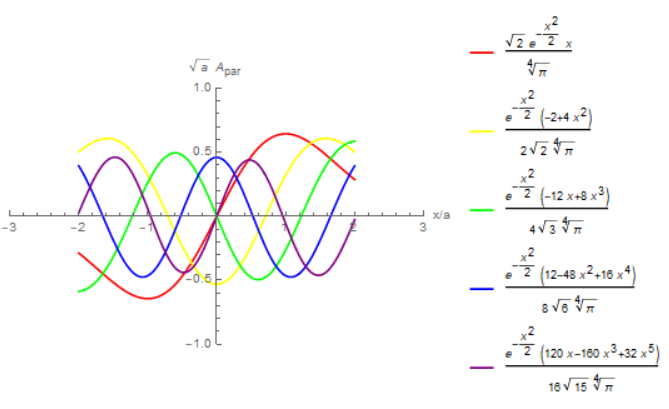
\includegraphics[width=0.8\textwidth]{Image/A_para.PNG}
        \caption{The growth rate peak of MTM with changing k}
        \label{fig:A_para}
\end{figure}



Integrate from both sides, we will be have

\begin{equation}
    \frac{dA}{dx}|^{x=l}_{x=-l} = \frac{4\pi}{c}\int ^{l}_{-l}dx j_{||}
\end{equation}

Since $\frac{1}{c^2}\frac{\partial ^2 }{\partial t^2} \sim k_{||}^2 \ll k^2$, then 

\begin{equation}
    \frac{d^2\textbf{A}_{||}}{dx^2} \approx \sigma(x) \textbf{A}_{||}
    \label{eq:A2}
\end{equation}

Where $\sigma(x)=\int\frac{\omega-\omega_*}{\omega - k_{||}v_{||}-i\nu}\frac{cq_sF_{0,s}}{T_s}v_{||}^2dv$

\subsection{Pertubation towards the exact solution}

From the quantized energy one can solve from quantuam mechanics: $E_n= (n+\frac{1}{2})\hbar \omega$, plug back into the transformation. 

\begin{equation}
    \sigma(0) +k_y^2 = (n+\frac{1}{2})\left[ 2 \sigma^{''}(0)\right]^{1/2}
\end{equation}



